\chapter{Theoretical Foundation}

If your work is based on other scientific theories and models, it is important to outline their structure and results. Use illustrations of models and theories as demonstrated below in Figure \ref{fig1}

\begin{figure}[H]
\centering
  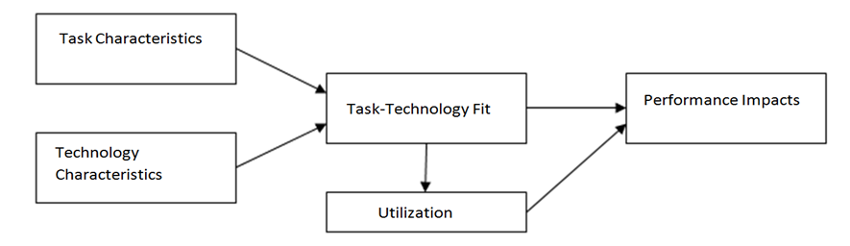
\includegraphics[width=1\textwidth]{grafiken/fig1}
   \caption{A picture of the universe!}
   \label{fig1}
\end{figure}


In addition to figures, one of the most powerful ways to present information in a coherent way is to create tables as shown in \ref{tab:table-name}. Make sure to include an empty line above tables and figures.
\begin{center}
\begin{table}[H]
\begin{tabularx}{\textwidth}{|X|X|X|}
\hline
Input & Output& Action return \\
\hline
DNF &  simulation & jsp\\
\hline
\end{tabularx}
\caption{\label{tab:table-name}Your caption.}
\end{table}
\end{center}


Multiple ways of presenting information can be chosen, e.g.

\begin{list}{•}{}
\item figures,
\item tables,
\item ordered lists,
\item and enumerations like this one. Here, items can be single sentences or full paragraphs. Appropriate end punctuation should be included.
\end{list}


\section{Citation Style}
Our chair suggests using the American Psychological Association (APA) 6th edition citation style. In order to give you insight into how to appropriately cite authors in your thesis, the following sections serve as a guideline. Adhering to the subsequent citation rules is vital to craft a successful and adequate paper. For clarification purposes, several examples referring to journal articles, conference papers, dissertations etcetera are given.
\section{Indirect Citations at the End of a Sentence}
If you write a statement or argument in your paper which is based on the idea or result from another author, you will have to cite the author at the end of the sentence. The citation style is not dependent on the type of publication (journal articles, conference papers, etc.), but rather determined by the number of authors.\\

\textbf{One author} 

The option to defer market entry and wait until market uncertainty is resolved can be valuable but risky \citep{fichman2004real}.\\

\textbf{Two authors}

Alignment bundles IT with other resources in a way that promotes consideration of how existing resources can be stretched to enhance current performance or how they can be used in new ways to prepare for change or to react to change \citep*{soh1995creates}.\\

\textbf{More than two authors}

Agility can improve performance by expanding a firm’s repertoire of competitive actions and the nature of its feasible responses to environmental change \citep*{lewis2003sources}. \\
\textit{Note: If you use a source multiple times in your thesis, make sure that the first reference contains every author’s name. Any following references should be shown in a shortened version naming the first author followed by “et al.”, an example could be: Agility can improve performance by expanding a firm’s repertoire of competitive actions and the nature of its feasible responses to environmental change \citep{lewis2003sources}.}
\section{Indirect Inline Citations}
If you highlight a result or an idea of authors, you can also use inline citations. Make sure that the reference is positioned close to the actual idea of the author(s).\\

\textbf{One author}

\cite{tallon2007process} reports that the primary locus of alignment within the firm (the process where alignment is highest) varies based on differences in strategic foci and so alignment is rarely the same in any two firms.\\

\textbf{Two authors}

Based on the results of our pilot study and comments from a panel of three IS academics, we adopted 12 of the 20 survey items used by \cite{terry2000measuring} to assess IT infrastructure flexibility: four items per construct.\\

\textbf{More than two authors}

As noted by \citet*{chin2003partial}, moderation can be modelled using a main and interaction effect; the main effect linking IT flexibility to agility does not need to be interpreted directly.

\section{Direct Citations}
Quotation marks are used to indicate that you are citing a complete thought. For these cases, page numbers need to be specified. These rules are applied, no matter what you cite (e.g. journals, conferences, books, and websites). The style for direct citations is demonstrated by the following examples:\\

\textbf{Direct citation of entire sentences}\\
``The recipe comprises necessary conditions and probabilistic processes in the following sequence: organizations spend on IT and, subject to the varying degrees of effectiveness during the IT management process, obtain IT assets. […] Favorable IT impacts, if not adversely affected during the competitive process, lead to improved organizational performance." \citep*[p.~39]{soh1995creates}.

\textit{Note: With “[…]” you highlight that you left out information originally contained in the citation but less relevant for your thesis. The meaning must not be changed by using this technique.}\\

\textbf{Direct citation of single information in a sentence}

The improvement of organizational performance can be achieved by creating “favorable IT impacts” \citep*[p.~39]{soh1995creates}.
\section{Footnotes}
We do not recommend the use of footnotes, however, if explanatory notes still prove necessary to your document, you can provide supplemental informationn\footnote{  See Soh \& Markus (1995) for an insightful analysis of information technology performance.}  in footnotes. When providing content notes, be brief and focus on only one subject. Try to limit your comments to one small paragraph. You can also point readers to information that is available in more detail elsewhere.



